\documentclass{article}
\usepackage[utf8]{inputenc}
\usepackage{graphicx}
\usepackage{amsmath}
\usepackage{caption}
\usepackage{hyperref}
\usepackage{geometry}
\geometry{margin=2.5cm}

\title{Percolation Project}
\author{Anaya Lizarazo, Bryan Johan; Pinilla Correa, Santiago \& Torres Otálora, Erick}
\date{\today}

\begin{document} 

\maketitle

\section{Introducción}

La percolación es un fenómeno físico y matemático que describe el comportamiento colectivo de elementos conectados en una red aleatoria. En este proyecto se estudia el modelo de percolación por sitios sobre una red cuadrada bidimensional de tamaño \( L \times L \). Este modelo consiste en recorrer cada uno de los sitios de la matriz y ocuparlo con una probabilidad \( p \). A partir de esta ocupación aleatoria, se identifican los conglomerados de sitios vecinos ocupados, conocidos como \emph{clusters}.

Para el reconocimiento eficiente de estos clusters se implementó el algoritmo de Hoshen-Kopelman, que permite etiquetar de manera rápida y sin redundancias los distintos conglomerados conectados de la matriz. Con esta información es posible determinar si existe un cluster que conecta los bordes opuestos de la red, es decir, si el sistema \emph{percola}.

En la figura \ref{fig:lattice_clusters} se ilustran dos representaciones de una red: una antes de identificar los clusters y otra después de aplicar el algoritmo de Hoshen-Kopelman, donde cada cluster ha sido etiquetado y representado con un color diferente.

\begin{figure}[h]
    \centering
    /%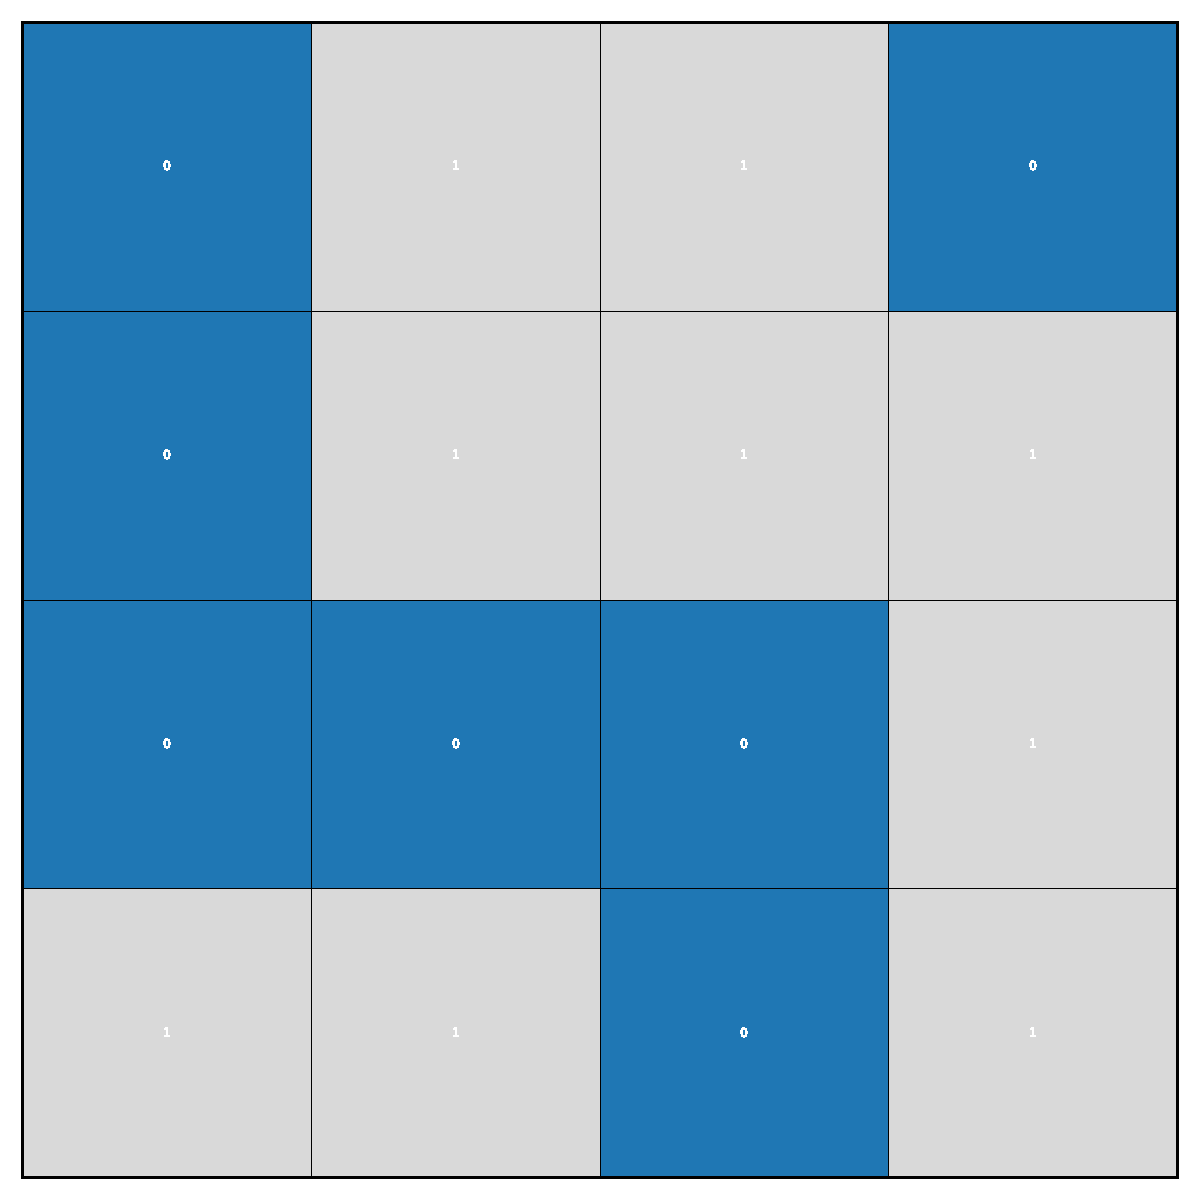
\includegraphics[width=0.45\textwidth]{lattice.pdf}
    \hfill
    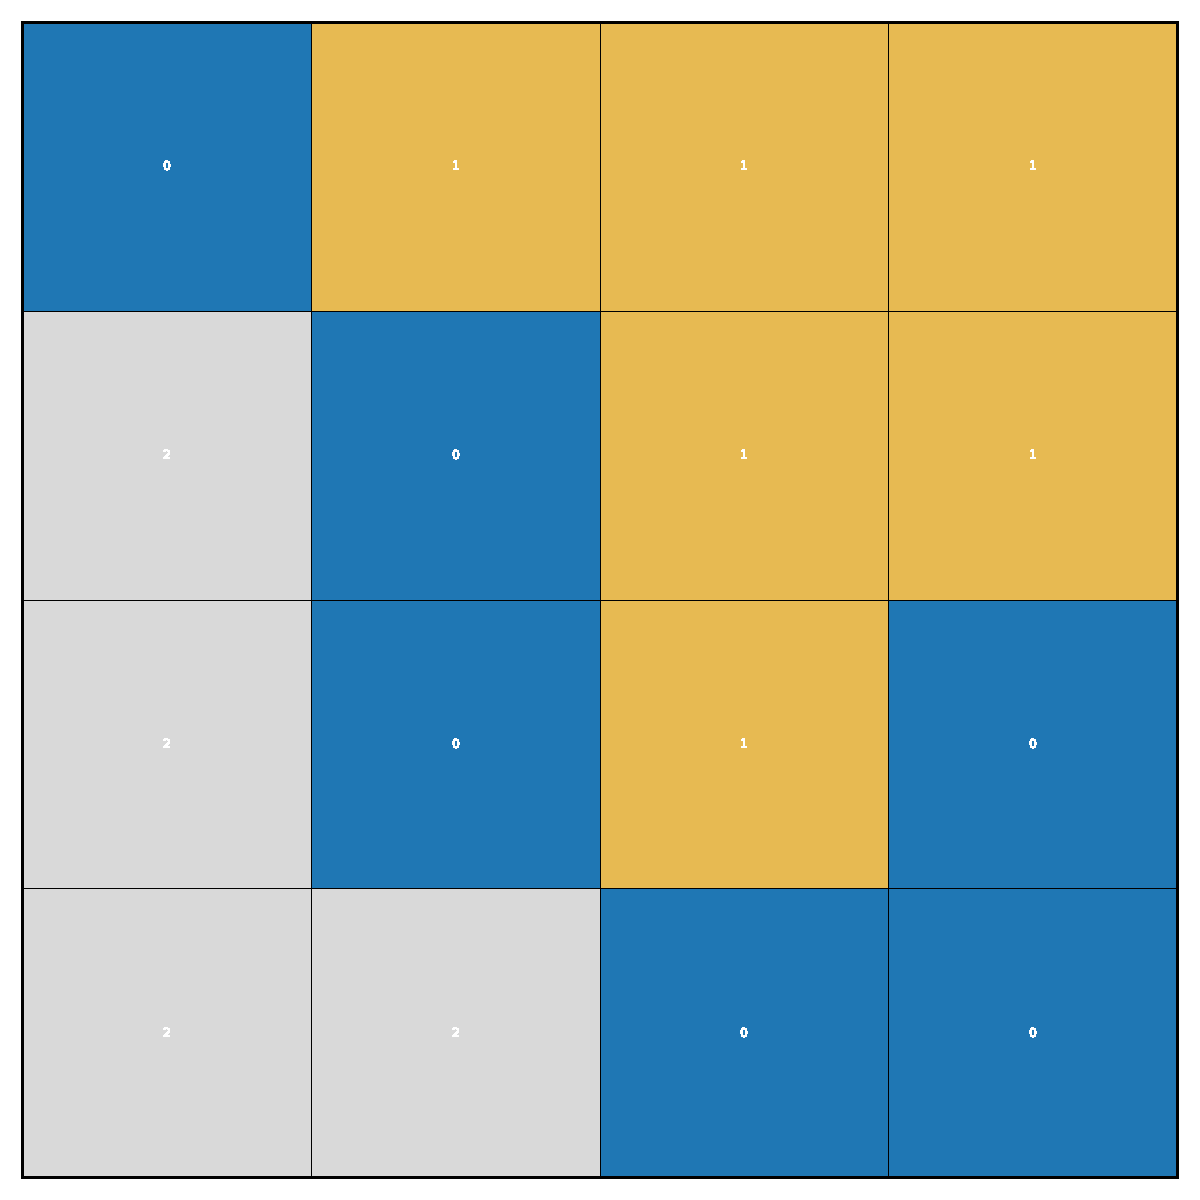
\includegraphics[width=0.45\textwidth]{figures/clusters.pdf}
    \caption{(Izquierda) Lattice de tamaño \( L \times L \) con ocupación aleatoria según probabilidad \( p \). (Derecha) Identificación de clusters mediante el algoritmo de Hoshen-Kopelman.}
    \label{fig:lattice_clusters}
\end{figure}
\section{Resultados}


\section{Conclusiones}
...

\end{document}
